% Analisi Matematica II, lezione 7: curve in R^n (definizione, sostegno, curve chiuse,
% semplici e regolari, esempi). Frammento da includere con \input; le figure
% figure/fig_NN.pdf sono generate da figure.py.

% [0:00:00]
\section{Che cos'è una curva?}

% [0:00:00]
La parola «curva» si usa di continuo e, trovandola in un testo di Analisi~II, quasi
nessuno si fermerebbe pensando di non conoscerne il significato. Eppure alla domanda
«che cos'è una curva?» le risposte spontanee non sono definizioni: «una linea non
retta» (ma allora una retta non può essere una curva?). Lo stesso accade chiedendo che
cos'è una traiettoria («l'insieme dei punti in cui il corpo è passato») o che cosa sono
una circonferenza e un'ellisse («una conica», «un luogo geometrico»).
% [0:02:16]
Sono tentativi un po' contorti di parlare di un oggetto che non è mai stato sistemato in
modo rigoroso e che si chiarisce solo in Analisi~II. Per esempio, l'ellisse si definisce
come luogo dei punti che verificano la proprietà dei fuochi, ma quando se ne scrive
l'equazione i fuochi spariscono: non sono il punto cruciale per descriverla.
% [0:03:19]
A scuola la questione non si può sistemare, perché servono funzioni particolari. La
risposta giusta, data da uno studente, è che una curva è una \emph{funzione}.

% [0:04:00]
\subsection{Traiettoria e legge oraria}

% [0:04:00]
Pensiamo a un punto che si muove di moto circolare, magari uniforme: la sua traiettoria,
diremmo, è una circonferenza. Se però un punto percorre la circonferenza una volta e un
altro la percorre cinque volte, il disegno è lo stesso (figura~\ref{fig:01}): hanno la
stessa traiettoria? Guardando solo la circonferenza non si vede quante volte è stata
percorsa: il luogo dei punti non tiene conto delle ripetizioni, e dalla sola figura non
si può risalire al moto.

\begin{figure}[htbp]\centering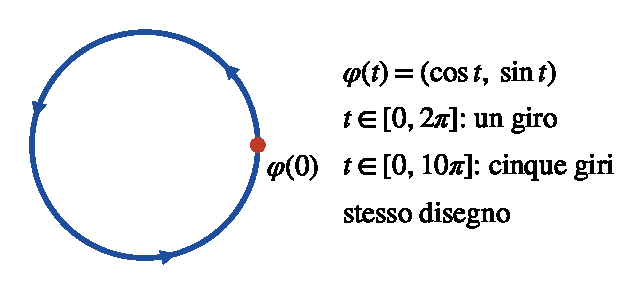
\includegraphics[width=0.6\linewidth]{figure/fig_01}\caption{La stessa circonferenza è l'immagine della legge oraria $\varphi(t)=(\cos t,\sin t)$ sia per $t\in[0,2\pi]$ (un giro) sia per $t\in[0,10\pi]$ (cinque giri): dal solo disegno non si distinguono i due moti.}\label{fig:01}\end{figure}

La circonferenza, da sola, non è dunque una traiettoria: dalle sole posizioni non si
distinguono moti diversi (dove si trovava il punto in un dato istante? quante volte l'ho percorsa? non posso
saperlo). Se si vuole chiamare la circonferenza «curva», bisogna assegnare una
\emph{legge oraria}: la curva è definita dall'applicazione che la determina.

% [0:05:22]
A chi obietta che, quando si studia la traiettoria, il tempo non interessa, si risponde
che proprio così la traiettoria resta associata a un'intera categoria di moti diversi.
Uno studente propone l'analogia con il piano complesso, dove aggiungendo un angolo giro
all'argomento si ritrova lo stesso punto: l'idea è proprio questa.

% [0:06:18]
Per distinguere i moti bisogna pensare la curva come dipendente da un parametro, il
tempo $t$, che dice istante per istante dove si trova il punto. La circonferenza è
allora l'\emph{immagine} della legge oraria:
% [0:07:17]
i due moti hanno la stessa immagine, ma le loro leggi orarie hanno domini diversi (a
parità di velocità, chi fa più giri ha avuto più tempo).

Se si vedono le curve attraverso le loro immagini, è più semplice capire che cosa accade
% [0:07:17]
quando si trova lo stesso sostegno su intervalli diversi; e il primo modo per capire
bene che cos'è una curva è ragionare come un fisico.
Pensiamo a una variabile, il tempo, a cui viene associata una posizione.

% [0:08:32]
\subsection{Dalle funzioni di Analisi~I alle curve}

% [0:08:32]
In Analisi~I si sono studiate le funzioni da $\mathbb{R}$ in $\mathbb{R}$. Poiché
$\mathbb{R}^n$ ha una struttura topologica (vi si possono fare i limiti), lo si può
mettere nel dominio, nel codominio o in entrambi:
\[
\mathbb{R}\to\mathbb{R}\ \Longrightarrow\ \text{Analisi I},
\qquad
\left.\begin{aligned}
&\mathbb{R}\to\mathbb{R}^n\\
&\mathbb{R}^n\to\mathbb{R}\\
&\mathbb{R}^n\to\mathbb{R}^m\quad(\text{per esempio i campi di forze})
\end{aligned}\right\}\ \text{Analisi II}.
\]
% [0:08:32]
Ognuna di queste classi ha un'interpretazione diversa e si studia in modo diverso. La
più familiare è $\mathbb{R}\to\mathbb{R}^n$: se $t$ è il tempo e a ogni istante si
associa una posizione, si ottiene la legge oraria di un moto, nota dalla scuola
secondaria. Per questo si parte da qui.

Partiamo dunque da $\mathbb{R}\to\mathbb{R}^n$: si ottiene un oggetto matematico nuovo,
% [0:09:59]
che non è più quello di Analisi~I e richiede una riflessione da Analisi~II.
Ciò che di solito chiamiamo «curva», cioè il disegno, è in realtà il \emph{sostegno}:
l'insieme dei punti, cioè l'immagine dell'applicazione.

\paragraph{In sintesi.} La traiettoria, intesa come disegno, è l'immagine; la
\emph{curva} è la legge oraria. Si possono avere due leggi orarie diverse con la stessa
immagine.
% [0:09:59]
La circonferenza della figura~\ref{fig:01} non è una curva: è l'immagine di una curva,
e ci sono infinite curve (leggi orarie) che l'hanno come immagine.
Non si può scindere il disegno dalla legge.

% [0:11:16]
Lo si vede pensando alla lunghezza. Se due moti avessero «la stessa traiettoria» solo
perché hanno lo stesso disegno, dovrebbero avere anche la stessa lunghezza percorsa, e
non è così.
% [0:12:18]
Intendendo la curva come legge oraria, invece, tutto torna: se la circonferenza è
percorsa una volta, la lunghezza della curva è il perimetro della circonferenza; se è
percorsa più volte, la lunghezza della curva conta tutti i giri. È giusto così, perché
la lunghezza è legata alla legge oraria.

Due curve possono dunque avere lo stesso disegno, la stessa circonferenza, ma domini
diversi: è l'esempio delle curve $\varphi_1$ e $\varphi_2$ della
sezione~\ref{sec:stesso-sostegno}.

% [0:12:18]
\paragraph{Osservazione.} Rispetto alla Fisica si troveranno alcune differenze di
linguaggio, per esempio fra «traiettoria» e «sostegno».
% [1:28:18]
Se qualcosa sembra non tornare fra Fisica e Analisi, conviene segnalarlo: di solito si
tratta di nomi diversi dati alla stessa cosa, come «centro di massa» e «baricentro».

% [0:14:20]
\section{Curve in $\mathbb{R}^n$}

% [0:14:20]
\subsection{Definizione di curva ed equazioni parametriche}

\paragraph{Definizione (curva).} Sia $\varphi\colon[a,b]\subset\mathbb{R}\to\mathbb{R}^n$
(oppure $\mathbb{R}^2$: curve piane),
\[
t\in[a,b]\ \longmapsto\ \varphi(t)=\bigl(x_1(t),x_2(t),\dots,x_n(t)\bigr)\in\mathbb{R}^n,
\]
dove ciascuna componente $x_i\colon[a,b]\to\mathbb{R}$ è continua. Quando tutte le $x_i$
sono continue, $\varphi$ è continua; allora $\varphi$ si chiama \emph{curva}. In
$\mathbb{R}^2$ si scrive $\varphi(t)=(x(t),y(t))$.

% [0:14:20]
$\varphi(t)$ è un vettore, il vettore posizione all'istante $t$, e le sue componenti sono
$x_1(t),\dots,x_n(t)$. Dove possibile si lavorerà in $\mathbb{R}^n$, per poi passare al
piano.
% [0:16:52]
Una curva è quindi una funzione continua da un intervallo di $\mathbb{R}$ in
$\mathbb{R}^n$; la si indica con una lettera greca (qui sempre $\varphi$).

% [0:15:49]
\paragraph{Osservazione (perché continua).} Un moto è discontinuo quando il punto, a un
certo istante, «salta» altrove: per esempio si ritrova di colpo a un altro piano
dell'edificio e poi riprende a camminare. In un caso del genere si studiano due moti
distinti, ciascuno continuo, su due intervalli di tempo diversi: se una traiettoria si
spezza, la si divide in due.
% [0:16:52]
Per questo nella definizione di curva si chiede subito la continuità.

\paragraph{Equazioni parametriche.} Le equazioni
\[
\varphi\colon\begin{cases}
x_1=x_1(t)\\
\quad\vdots\\
x_n=x_n(t)
\end{cases}
\qquad t\in[a,b],
\]
si chiamano \emph{equazioni parametriche} della curva. Si possono scrivere anche in riga,
$\varphi(t)=(x_1(t),\dots,x_n(t))$:
% [0:17:37]
nell'uno e nell'altro modo si dice quali sono le funzioni componenti, cioè si assegna la
curva.

% [0:19:03]
\subsection{Sostegno, punto iniziale e finale, curve chiuse}

\paragraph{Definizione (sostegno).} Si chiama \emph{sostegno} della curva la sua
immagine, cioè l'insieme
\[
\varphi([a,b])=\{\varphi(t):t\in[a,b]\}\subset\mathbb{R}^n.
\]
La traiettoria è il sostegno:
% [0:19:03]
è il «disegno», l'insieme di tutte le posizioni occupate.

\paragraph{Definizione (punto iniziale e finale, curva chiusa).} I punti $\varphi(a)$ e
$\varphi(b)$ si chiamano \emph{punto iniziale} e \emph{punto finale} della curva. Una
curva si dice \emph{chiusa} se $\varphi(a)=\varphi(b)$.

Le curve chiuse sono importanti nello studio dei campi conservativi.
% [0:20:27]
In Fisica la conservatività di un campo si collega alla circuitazione lungo i percorsi
chiusi; questo legame andrà precisato, perché certe condizioni valgono per alcuni campi
e non per tutti. In Fisica funzionavano perché si consideravano soprattutto
gradienti, per lo più campi radiali definiti a meno di un punto.

% [0:21:13]
\subsection{Curve diverse con lo stesso sostegno}\label{sec:stesso-sostegno}

\paragraph{Esempio.} Consideriamo
\[
\varphi_1\colon[0,2\pi]\to\mathbb{R}^2,\quad \varphi_1(t)=(\cos t,\sin t);
\qquad
\varphi_2\colon[0,3\pi]\to\mathbb{R}^2,\quad \varphi_2(t)=(\cos t,\sin t).
\]
% [0:22:21]
Per riconoscere il sostegno basta elevare al quadrato le componenti e sommarle:
$\cos^2t+\sin^2t=1$, quindi i punti stanno sulla circonferenza di centro l'origine e
raggio~$1$.
Questa circonferenza è il sostegno sia di $\varphi_1$ sia di $\varphi_2$
(figura~\ref{fig:02}), ma le due curve hanno domini diversi. Dal punto di vista del
sostegno sono identiche, eppure sono due curve diverse:
% [0:23:36]
$\varphi_1$ fa un giro completo, partendo da $(1,0)$ e tornandoci, mentre $\varphi_2$ fa
mezzo giro in più.

\begin{figure}[htbp]\centering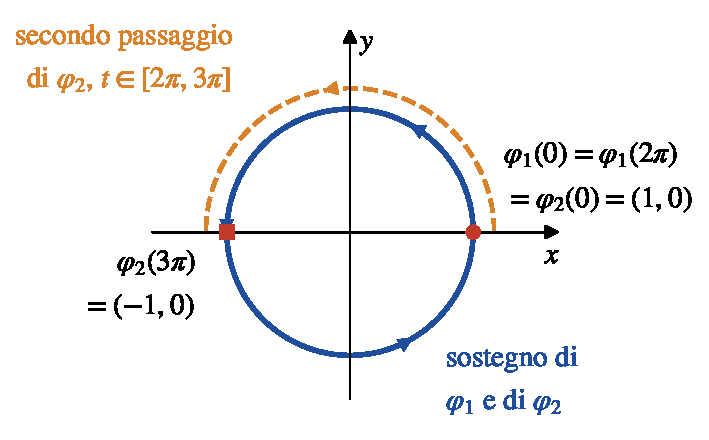
\includegraphics[width=0.6\linewidth]{figure/fig_02}\caption{Le curve $\varphi_1$ (su $[0,2\pi]$) e $\varphi_2$ (su $[0,3\pi]$) hanno lo stesso sostegno, la circonferenza unitaria. $\varphi_1$ parte e arriva in $(1,0)$; $\varphi_2$ parte da $(1,0)$, fa mezzo giro in più e termina in $(-1,0)$: il tratteggio, disegnato un po' all'esterno per renderlo visibile, è il suo secondo passaggio sulla semicirconferenza superiore.}\label{fig:02}\end{figure}

\paragraph{Osservazione.} Due curve che hanno lo stesso sostegno non sono necessariamente
la stessa curva. Infatti $\varphi_1$ è chiusa, perché $\varphi_1(0)=\varphi_1(2\pi)=(1,0)$,
mentre $\varphi_2$ è aperta: $\varphi_2(0)=(1,0)\neq(-1,0)=\varphi_2(3\pi)$.
% [0:25:03]
Se si calcolasse la circuitazione guardando solo l'insieme, cioè la circonferenza, si
sbaglierebbe: $\varphi_2$ non è nemmeno chiusa.

\paragraph{Osservazione.} Il sostegno, cioè il disegno (la traiettoria), non identifica
l'applicazione, cioè la curva.
% [0:25:03]
È un fatto che deve lasciare un po' interdetti: in Analisi~I la teoria delle funzioni si
basa sul fatto che il grafico identifica la funzione (dal grafico si ricava tutto sulla
funzione e, viceversa, la funzione determina il grafico). Qui non è così: il sostegno
non è un grafico. L'argomento sembra facile perché le leggi orarie sono familiari, ma
dal punto di vista matematico le differenze rispetto ad Analisi~I sono notevoli.
% [0:26:15]
Conviene quindi segnarsi sempre da dove si parte e dove si arriva. Nell'ottica delle
curve, inoltre, circonferenza, ellisse e iperbole si possono definire senza chiamare in
causa i fuochi e senza le dimostrazioni che a scuola portano all'equazione canonica (per
circonferenza ed ellisse si vedano gli esempi~2 e~3 della sezione~\ref{sec:esempi}).

% [0:27:36]
\section{Curve semplici e curve regolari}

% [0:27:36]
\subsection{Curve semplici}

\paragraph{Definizione (curva semplice).} Una curva $\varphi\colon[a,b]\to\mathbb{R}^n$ si
dice \emph{semplice} se
\[
\forall\,t_1\neq t_2,\ \text{con almeno uno dei due interno ad }[a,b],\quad
\text{risulta}\quad \varphi(t_1)\neq\varphi(t_2).
\]
% [0:31:56]
«Interno ad $[a,b]$» significa appartenente all'intervallo aperto $]a,b[$.
% [0:28:41]
Nei moti visti in Fisica le leggi orarie sono di solito semplici: raramente si
considerano moti che si incrociano.

\paragraph{Esempio.} Riprendiamo le curve precedenti e aggiungiamo la curva
$\varphi_3(t)=(\cos t,\sin t)$, con $t\in[0,4\pi]$.
\begin{itemize}
\item La circonferenza $\varphi_2$, percorsa su $[0,3\pi]$, non è chiusa e non è semplice:
% [0:28:41]
facendo mezzo giro in più, i punti della semicirconferenza superiore sono occupati sia
negli istanti $t\in[0,\pi]$ sia negli istanti $t\in[2\pi,3\pi]$.
\item $\varphi_1$ è chiusa e semplice:
% [0:28:41]
torna nella posizione iniziale, ma per una curva semplice «tornare a casa» è consentito.
Le curve chiuse, dunque, possono essere semplici.
\item $\varphi_3$ è chiusa ma non semplice:
% [0:30:53]
facendo due giri, occupa di nuovo tutte le stesse posizioni negli istanti fra $2\pi$ e
$4\pi$.
\end{itemize}

\begin{center}
\begin{tabular}{cccc}
\hline
curva & intervallo & chiusa & semplice\\
\hline
$\varphi_1$ & $[0,2\pi]$ & sì & sì\\
$\varphi_2$ & $[0,3\pi]$ & no & no\\
$\varphi_3$ & $[0,4\pi]$ & sì & no\\
\hline
\end{tabular}
\end{center}

% [0:31:56]
\paragraph{Osservazione (perché $\varphi_1$ è semplice).} Pensiamo a $t$ come all'angolo:
il punto parte da $t=0$, si muove e arriva a $t=2\pi$, e nel giro di $360^\circ$ occupa
sempre posizioni diverse; solo alla fine $\varphi_1(0)=\varphi_1(2\pi)$. La definizione
lo consente: gli istanti $t_1=0$ e $t_2=2\pi$ sono diversi, ma nessuno dei due è interno
all'intervallo, quindi la condizione non li riguarda.
% [0:33:26]
La curva può chiudersi, ma poi non deve più muoversi: basta un $\varepsilon$ di angolo in
più e non è più semplice. Le curve semplici hanno inoltre questa particolarità: quando
se ne calcola la lunghezza, si ottiene proprio il percorso fatto, senza tratti ripetuti.

% [0:33:26]
\paragraph{Esempio.} La curva $t\mapsto(t,t^2)$ è semplice (e non chiusa) su $[0,500]$,
% [0:34:50]
ma anche su $[-50,50]$: benché $t^2$ assuma lo stesso valore in $t$ e in $-t$, la prima
componente $t$ distingue sempre gli istanti.

\paragraph{Osservazione.} La definizione di curva semplice è un modo per «inventarsi» una
definizione di iniettività, consentendo a un punto materiale di «ritornare» all'inizio.
% [0:34:50]
L'iniettività di Analisi~I non si può usare così com'è: escluderebbe proprio i punti che
tornano a casa, cioè le curve chiuse.

% [0:34:50]
\subsection{Curve regolari, vettore e versore tangente}

\paragraph{Definizione (curva regolare).} Una curva $\varphi\colon[a,b]\to\mathbb{R}^n$ si
dice \emph{regolare} se:
\begin{enumerate}
\item $\varphi\in C^1(]a,b[)$;
\item posto $\varphi'(t)=\bigl(x_1'(t),\dots,x_n'(t)\bigr)$, si ha
$\varphi'(t)\neq(0,\dots,0)$ per ogni $t\in\,]a,b[$, ovvero $|\varphi'(t)|>0$ per ogni
$t\in\,]a,b[$.
\end{enumerate}
In altre parole, deve essere sempre possibile calcolare una velocità di modulo non
nullo.
% [0:36:17]
La condizione~1 significa che $\varphi$ è derivabile in tutti i punti interni, con
derivata continua; la derivata di $\varphi$ è il vettore delle derivate delle componenti.
Entrambe le condizioni si verificano sull'intervallo aperto.

\paragraph{Definizione (vettore e versore tangente).} Il vettore $\varphi'(t)$ si chiama
\emph{vettore tangente} alla curva; il \emph{versore tangente} è
\[
T(t)=\frac{\varphi'(t)}{|\varphi'(t)|}.
\]
% [0:37:29]
Il modulo non nullo si richiede proprio per poter definire il versore tangente: per una
curva regolare $|\varphi'(t)|\neq0$ e la frazione ha senso. Il versore $T(t)$ ha norma
$|T(t)|=1$ e indica direzione e verso istantanei del moto.

% [0:38:30]
La figura~\ref{fig:03} illustra la situazione: $\varphi$ porta l'intervallo $[a,b]$ in una
curva del piano, dal punto iniziale $\varphi(a)$ al punto finale $\varphi(b)$, e in ogni
istante si può tracciare il versore tangente (il disegno è più chiaro con una curva che
non si chiude). Pensando al moto, $\varphi'(t)$ è la velocità: ecco perché la velocità ha
la direzione della tangente alla traiettoria.

\begin{figure}[htbp]\centering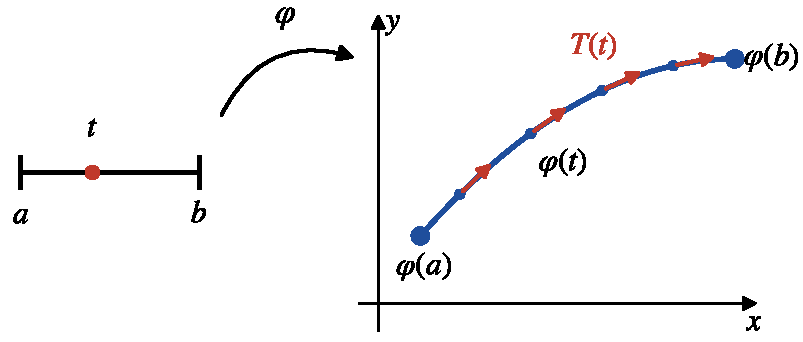
\includegraphics[width=0.6\linewidth]{figure/fig_03}\caption{Una curva regolare $\varphi\colon[a,b]\to\mathbb{R}^2$: l'intervallo $[a,b]$ viene portato in una curva del piano che va da $\varphi(a)$ a $\varphi(b)$; in rosso il versore tangente $T(t)$ in alcuni istanti (andamento qualitativo).}\label{fig:03}\end{figure}

% [0:39:46]
\subsection{Perché studiamo le curve}

Dall'Analisi~I è rimasta una questione in sospeso: calcolare il perimetro, cioè la
lunghezza, dei grafici. Con le curve chiuderemo la questione degli integrali.

% [0:39:46]
Il grafico di una funzione $y=f(x)$ si può riguardare come una curva, quella che associa
a $x$ la posizione $(x,f(x))$ (esempio~1 della sezione~\ref{sec:esempi}). Con
l'integrale ci si è posti il problema di calcolare le aree dei rettangoloidi;
% [0:40:57]
a scuola, invece, l'ordine era l'opposto: prima i perimetri (le lunghezze, grandezze di
dimensione~1), poi le superfici e, in terza media, i volumi. Il problema di calcolare la
lunghezza del grafico, e quindi il perimetro del rettangoloide, richiede l'Analisi~II, perché
bisogna prima capire che oggetto è il grafico: una curva. L'obiettivo finale di questo
argomento è calcolare le lunghezze delle curve; così, per queste figure, si sapranno
calcolare sia l'area sia il perimetro.

% [0:42:09]
\paragraph{Cenno storico.} Le curve servono anche a risolvere problemi che con la sola
riga e il solo compasso non si possono risolvere. I Greci si posero tre problemi di
costruzione con riga e compasso: la \emph{duplicazione del cubo} (dato un cubo,
costruirne uno di volume doppio), la \emph{trisezione dell'angolo} (dividere un angolo
qualsiasi in tre parti uguali) e la \emph{quadratura del cerchio} (dato un cerchio,
costruire un quadrato con la stessa area).
% [0:43:38]
Con la sola riga e il solo compasso nessuno dei tre si può risolvere (così come non si
può costruire l'eptagono regolare, a differenza dell'esagono e dell'ottagono); sono stati
risolti ricorrendo a curve particolari, costruite ad hoc.

% [0:47:47]
\section{Esempi di curve}\label{sec:esempi}

% [0:47:47]
Gli esempi sono in $\mathbb{R}^2$ e in $\mathbb{R}^3$. Per ciascuno ci si chiede se la
curva è chiusa, se è semplice e se è regolare.

% [0:47:47]
\subsection{Esempio 1: curva cartesiana}

Sia $f\colon[a,b]\to\mathbb{R}$, con $f\in C^1([a,b])$
% [0:47:47]
(una funzione di Analisi~I, non una curva).
Si chiama \emph{curva cartesiana} la curva
\[
\varphi\colon t\in[a,b]\ \longmapsto\ \varphi(t)=(t,f(t))\in\mathbb{R}^2,
\qquad\text{cioè}\qquad
\varphi\colon\begin{cases} x=t\\ y=f(t)\end{cases}
\]
(equazioni parametriche di una curva in $\mathbb{R}^2$). Poiché $f\in C^1$, si possono
fare alcune osservazioni. Innanzitutto il sostegno è il grafico di $f$
(figura~\ref{fig:04}):
% [0:49:09]
il sostegno è l'insieme delle coppie $(t,f(t))$, cioè proprio il grafico. Fra tutte le
curve, i grafici sono la classe che ci interessa: sono quelli che vogliamo imparare a
misurare.

\begin{figure}[htbp]\centering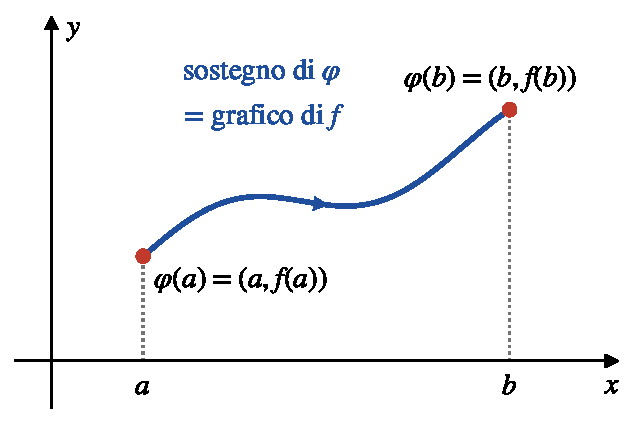
\includegraphics[width=0.6\linewidth]{figure/fig_04}\caption{Curva cartesiana $\varphi(t)=(t,f(t))$, $t\in[a,b]$: il sostegno è il grafico di $f$ (andamento qualitativo).}\label{fig:04}\end{figure}

\paragraph{Proprietà.}
\begin{enumerate}
\item Non è chiusa: se si chiudesse, perderebbe la definizione di funzione.
% [0:50:36]
La prima componente $t$ cambia sempre, quindi $\varphi(a)=(a,f(a))$ e
$\varphi(b)=(b,f(b))$ non possono coincidere.
\item È ovviamente semplice:
% [0:50:36]
per avere la stessa coppia bisogna avere lo stesso $t$.
\item È regolare, perché $\varphi'(t)=(1,f'(t))$ e
\[
|\varphi'(t)|=\sqrt{1+f'(t)^2}\ge1>0\qquad\forall\,t\in[a,b]
\]
% [0:50:36]
(addirittura sull'intervallo chiuso).
\end{enumerate}
% [0:50:36]
È un esempio di curva «buonissima», che però non si chiude mai.

% [0:51:53]
\subsection{Esempio 2: circonferenza}

Sia $\varphi\colon[0,2\pi]\to\mathbb{R}^2$ definita da
\[
\varphi\colon\begin{cases} x(t)=x_0+R\cos t\\ y(t)=y_0+R\sin t\end{cases}
\qquad t\in[0,2\pi],
\]
dove $(x_0,y_0)\in\mathbb{R}^2$ e $R>0$. Il sostegno è la circonferenza di centro
$(x_0,y_0)$ e raggio $R$ (figura~\ref{fig:05}):
\[
(x-x_0)^2+(y-y_0)^2=R^2.
\]
% [0:53:31]
Infatti, sostituendo a $x$ e a $y$ le componenti, si ottiene
$R^2\cos^2t+R^2\sin^2t=R^2$.

\begin{figure}[htbp]\centering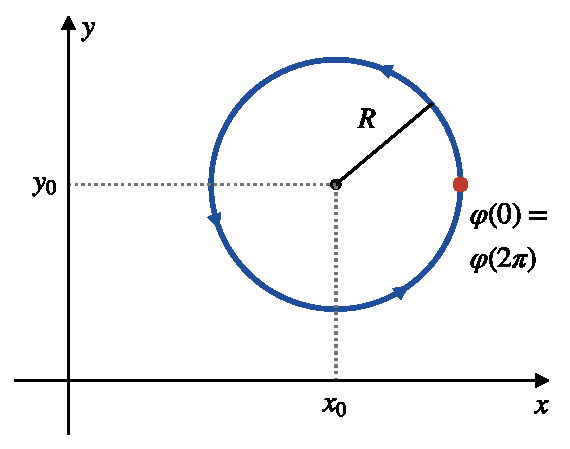
\includegraphics[width=0.6\linewidth]{figure/fig_05}\caption{Sostegno della circonferenza $\varphi(t)=(x_0+R\cos t,\ y_0+R\sin t)$, $t\in[0,2\pi]$: centro $(x_0,y_0)$ e raggio $R$; le frecce indicano il verso di percorrenza.}\label{fig:05}\end{figure}

\paragraph{Proprietà.}
\begin{enumerate}
\item È chiusa:
% [0:54:41]
per come è stato scelto l'intervallo, $\varphi(0)=\varphi(2\pi)=(x_0+R,\,y_0)$.
\item È semplice:
% [0:54:41]
non si autointerseca; istanti diversi danno punti diversi, tranne la coppia di estremi
$t=0$, $t=2\pi$, che la definizione consente. Infatti, presi $t_1,t_2\in[0,2\pi[$, la
condizione $\varphi(t_1)=\varphi(t_2)$ richiede
\[
\begin{cases}\cos t_1=\cos t_2\\ \sin t_1=\sin t_2\end{cases}
\iff t_1-t_2=2k\pi,\quad k\in\mathbb{Z},
\]
e nell'intervallo $[0,2\pi[$ l'unica possibilità è $k=0$, cioè $t_1=t_2$.
\item È regolare:
% [0:54:41]
derivando le componenti (le costanti $x_0$ e $y_0$ spariscono) si ha
\[
\varphi'(t)=(-R\sin t,\ R\cos t),\qquad
|\varphi'(t)|=\sqrt{R^2\sin^2t+R^2\cos^2t}=R>0\quad\forall\,t\in\,]0,2\pi[.
\]
\end{enumerate}
% [0:55:28]
Il modulo $|\varphi'(t)|$ servirà più avanti (chi ha già visto l'ascissa curvilinea lo
sa).
% [0:56:34]
Se si allarga l'intervallo oltre $[0,2\pi]$, il sostegno non cambia e succede quanto
visto con $\varphi_2$ e $\varphi_3$.

% [0:56:34]
\subsection{Esempio 3: ellisse}

Sia $\varphi\colon[0,2\pi]\to\mathbb{R}^2$ definita come segue:
\[
\varphi\colon\begin{cases} x(t)=x_0+a\cos t\\ y(t)=y_0+b\sin t\end{cases}
\qquad t\in[0,2\pi],
\]
dove $(x_0,y_0)\in\mathbb{R}^2$ e $a,b>0$ si chiamano \emph{semiassi} (qui $a$ e $b$ non
sono gli estremi dell'intervallo). Il sostegno è l'ellisse
\[
\frac{(x-x_0)^2}{a^2}+\frac{(y-y_0)^2}{b^2}=1.
\]
% [0:58:03]
Infatti, togliendo $x_0$ alla prima componente, elevando al quadrato e dividendo per
$a^2$ resta $\cos^2t$; facendo lo stesso con la seconda (togliere $y_0$, dividere per
$b^2$) resta $\sin^2t$, e la somma vale~$1$. È l'analogo dell'equazione vista a scuola,
ottenuto senza passare per i fuochi.

Ci sono due tipi di sostegno, $a>b$ e $b>a$ (figura~\ref{fig:06}):
% [0:59:20]
nel primo caso si ha una specie di uovo disteso, di centro $(x_0,y_0)$, con il semiasse
orizzontale $a$ più lungo di quello verticale $b$; nel secondo l'ellisse è disposta in
verticale. Nel caso particolare $a=b=R$ si ritrova la circonferenza di raggio $R$
dell'esempio~2.

\begin{figure}[htbp]\centering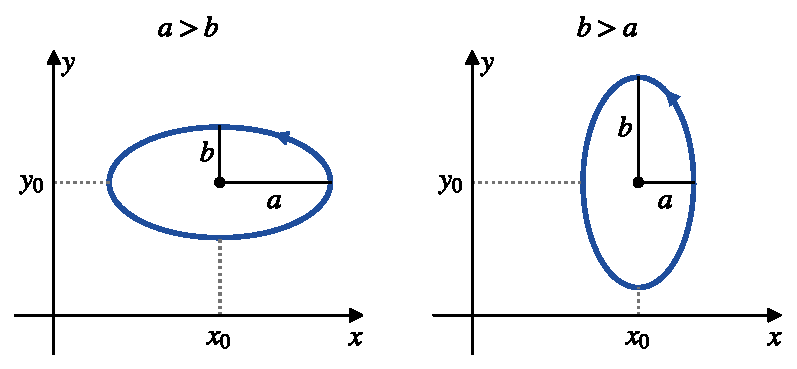
\includegraphics[width=0.6\linewidth]{figure/fig_06}\caption{Sostegno dell'ellisse $\varphi(t)=(x_0+a\cos t,\ y_0+b\sin t)$ nei due casi $a>b$ (a sinistra, con $a=2$, $b=1$) e $b>a$ (a destra, con $a=1$, $b=1{,}9$).}\label{fig:06}\end{figure}

\paragraph{Proprietà.}
\begin{enumerate}
\item È chiusa: $\varphi(0)=\varphi(2\pi)=(x_0+a,\,y_0)$.
\item È semplice
% [1:00:26]
(fa un solo giro): come per la circonferenza, presi $t_1,t_2\in[0,2\pi[$, l'uguaglianza
$\varphi(t_1)=\varphi(t_2)$ impone $\cos t_1=\cos t_2$ e $\sin t_1=\sin t_2$, quindi
$t_1=t_2$.
\item È regolare:
\[
\varphi'(t)=(-a\sin t,\ b\cos t),\qquad
|\varphi'(t)|^2=a^2\sin^2t+b^2\cos^2t>0,
\]
% [1:00:26]
perché seno e coseno non si annullano mai contemporaneamente.
\end{enumerate}

% [1:01:23]
\subsection{Esempio 4: una curva regolare ma non semplice}

Studiamo la curva
\[
\varphi(t)=\bigl(-t^3-2t^2-t,\ t^3+t^2\bigr),\qquad t\in[-a,a],\quad a>1.
\]
% [1:02:54]
Si prende un intervallo compatto centrato in $0$ che contenga $-1$ al suo interno: per
questo $a>1$. Conviene scrivere le componenti in forma fattorizzata:
\[
x(t)=-t(t+1)^2,\qquad y(t)=t^2(t+1).
\]

\paragraph{1) È chiusa?} Bisogna confrontare $\varphi(-a)$ e $\varphi(a)$: sono diversi,
quindi la curva non è chiusa.
% [1:03:49]
Basta guardare la seconda componente: in $t=-a$ vale $-a^3+a^2=a^2(1-a)<0$, mentre in
$t=a$ vale $a^3+a^2>0$.

\paragraph{2) Non è semplice.} Si ha $\varphi(0)=\varphi(-1)=(0,0)$.
% [1:05:16]
Lo si trova studiando gli zeri: la seconda componente è $t^3+t^2=t^2(t+1)$, che si
annulla in $t=0$ e in $t=-1$; sostituendo questi valori nella prima componente si
ottiene ancora $0$ (per $t=-1$: $1-2+1=0$). Dunque in due istanti diversi, entrambi
interni a $[-a,a]$, il punto occupa la stessa posizione: passa per l'origine una prima
volta per $t=-1$ e di nuovo per $t=0$.
% [1:06:44]
In generale si procede come per l'iniettività in Analisi~I, dove si poneva
$f(x_1)=f(x_2)$: si impone $\varphi(t_1)=\varphi(t_2)$ componente per componente e si
cercano soluzioni con $t_1\neq t_2$ e almeno uno dei due istanti interno all'intervallo.
Se non ce ne sono (o se l'unica coppia è quella dei due estremi), la curva è semplice.

\paragraph{3) È regolare?} Si ha
\[
\varphi'(t)=\bigl(-3t^2-4t-1,\ 3t^2+2t\bigr).
\]
Può essere il vettore nullo? Conviene partire dagli zeri della seconda componente:
\[
3t^2+2t=t(3t+2)=0\iff t=0\ \ \text{oppure}\ \ t=-\tfrac23 .
\]
I suoi zeri annullano anche la prima componente? No:
% [1:09:18]
in $t=0$ la prima componente vale $-1$, in $t=-\frac23$ vale
$-\frac43+\frac83-1=\frac13$. Quindi $\varphi'(t)\neq(0,0)$ per ogni $t$ e la curva è
regolare.

È dunque un esempio di curva non semplice ma regolare, come la circonferenza $\varphi_2$
percorsa su $[0,3\pi]$.
% [1:09:18]
Semplicità e regolarità sono proprietà indipendenti l'una dall'altra: la regolarità è una
proprietà locale (in ogni istante la velocità è non nulla e la tangente è ben definita),
la semplicità è una proprietà globale (il sostegno non si autointerseca).

Quando una curva non è semplice, si attorciglia su se stessa:
% [1:10:12]
disegnandola (figura~\ref{fig:07}) si vede che per l'origine si passa due volte, in due
istanti diversi.

\begin{figure}[htbp]\centering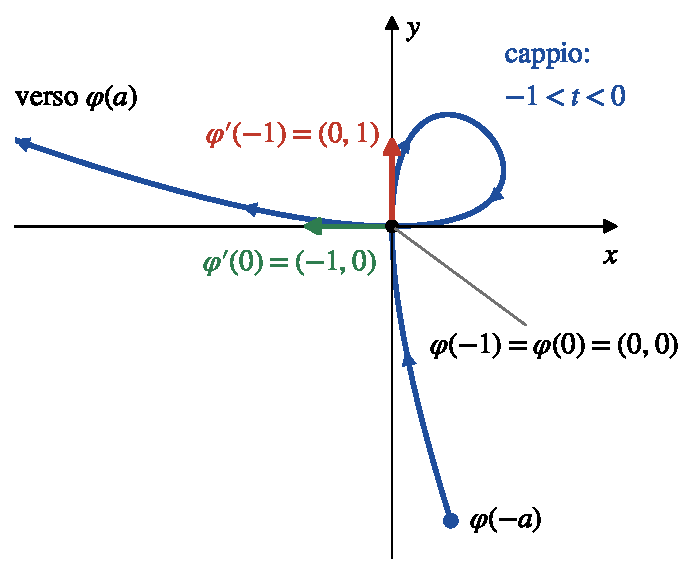
\includegraphics[width=0.6\linewidth]{figure/fig_07}\caption{La curva $\varphi(t)=(-t^3-2t^2-t,\ t^3+t^2)$ vicino all'origine, con $a=1{,}25$: il punto parte da $\varphi(-a)$ nel quarto quadrante, passa per l'origine in $t=-1$ con velocità $(0,1)$, percorre il cappio nel primo quadrante e ripassa per l'origine in $t=0$ con velocità $(-1,0)$; il ramo per $t>0$ prosegue fuori dal riquadro fino a $\varphi(a)$.}\label{fig:07}\end{figure}

\paragraph{Verso di percorrenza.} Da dove la percorriamo?
% [1:11:24]
Bisogna guardare la velocità $\varphi'$ nei due istanti in cui il punto passa per
l'origine, $t=-1$ e $t=0$ (non è nulla, perché la curva è regolare):
\[
\varphi'(-1)=(0,1),\qquad \varphi'(0)=(-1,0).
\]
% [1:13:39]
Poiché $-1$ precede $0$: all'istante $t=-1$ il punto attraversa l'origine con velocità
verticale, diretta verso l'alto come l'asse $y$; percorre poi il cappio nel primo
quadrante e all'istante $t=0$ ripassa per l'origine con velocità diretta verso sinistra,
nel verso opposto all'asse $x$ (frecce nella figura~\ref{fig:07}). Dalla forma
fattorizzata delle componenti si ricava in quali quadranti si trova il punto:
\begin{itemize}
\item per $t<-1$: $x(t)>0$ e $y(t)<0$, quarto quadrante;
\item per $-1<t<0$: $x(t)>0$ e $y(t)>0$, quindi il cappio è tutto nel primo quadrante;
\item per $t>0$: $x(t)<0$ e $y(t)>0$, secondo quadrante, dove la curva si allontana verso
l'alto a sinistra.
\end{itemize}

% [1:15:39]
\subsection{Esempio 5: cuspide}

Sia $\varphi(t)=(t^3,t^2)$, con $t\in[-1,1]$: è un esempio di curva non regolare
(figura~\ref{fig:08}).
% [1:15:39]
La forma del sostegno, la cuspide, ricorda i punti di non derivabilità di Analisi~I: ci
si aspetta che lì manchi il vettore tangente.
\begin{enumerate}
\item Non è chiusa: $\varphi(-1)=(-1,1)\neq(1,1)=\varphi(1)$.
\item È semplice, perché $t^3$ è iniettiva
% [1:15:39]
(se una delle funzioni componenti è iniettiva, la curva è semplice).
\item Non è regolare: l'origine è un punto «di non derivabilità» del sostegno. Infatti
\[
\varphi'(t)=(3t^2,\ 2t)=(0,0)\quad\text{se } t=0,
\]
e $t=0$ è interno a $[-1,1]$: la curva non è regolare in $t=0$. (La funzione $\varphi$ è
derivabile anche in $t=0$: a mancare è il versore tangente, perché $\varphi'(0)$ è il
vettore nullo.)
\end{enumerate}
Eliminando il parametro si ritrova il grafico di una funzione di Analisi~I: da $x=t^3$ si
ha $t=\sqrt[3]{x}$ e quindi
\[
y=x^{2/3}=\sqrt[3]{x^2},
\]
che nell'origine ha un punto di non derivabilità a tangente verticale (derivata destra
$+\infty$, sinistra $-\infty$), cioè una cuspide.
% [1:17:05]
È la forma con cui da bambini si disegnano le rondini.

\begin{figure}[htbp]\centering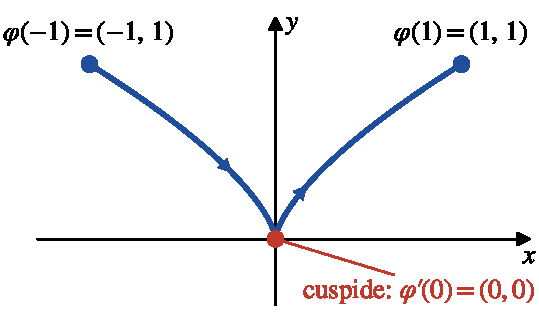
\includegraphics[width=0.6\linewidth]{figure/fig_08}\caption{Cuspide $\varphi(t)=(t^3,t^2)$, $t\in[-1,1]$, percorsa da $\varphi(-1)$ a $\varphi(1)$: nell'origine $\varphi'(0)=(0,0)$ e la curva non è regolare.}\label{fig:08}\end{figure}

% [1:18:01]
\subsection{Esempio 6: cicloide}

\[
\varphi\colon\begin{cases} x(t)=r\,(t-\sin t)\\ y(t)=r\,(1-\cos t)\end{cases}
\qquad t\in[0,2\pi],\quad r>0.
\]
% [1:18:01]
Si immagina una ruota di raggio $r$ che rotola senza strisciare su una retta (il piano
della cattedra) e si segue la posizione di un suo punto, per esempio quello inizialmente
appoggiato. Il punto torna sulla retta quando la ruota ha fatto un giro completo, e poi
il moto ricomincia: fermandosi a $t\in[0,2\pi]$ si vede un solo arco;
% [1:19:16]
proseguendo se ne ottengono altri, che toccano la retta nei punti di ascissa $2\pi r$,
$4\pi r$, \dots, cioè dopo tratti pari alla lunghezza della circonferenza della ruota
(figura~\ref{fig:09}). Le equazioni si ricavano dall'analisi cinematica del problema;
qui interessano le proprietà matematiche della curva.

\begin{figure}[htbp]\centering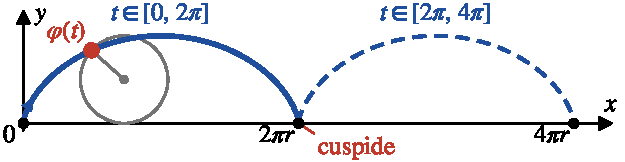
\includegraphics[width=0.6\linewidth]{figure/fig_09}\caption{Cicloide con $r=1$: l'arco per $t\in[0,2\pi]$ (tratto continuo), descritto dal punto $\varphi(t)$ della ruota che rotola sulla retta, e la prosecuzione per $t\in[2\pi,4\pi]$ (tratteggio); in $(2\pi r,0)$ si forma una cuspide.}\label{fig:09}\end{figure}

\begin{enumerate}
\item Non è chiusa:
% [1:19:16]
$\varphi(0)=(0,0)\neq(2\pi r,0)=\varphi(2\pi)$.
\item È semplice:
% [1:20:41]
la prima componente $r(t-\sin t)$ assume valori diversi in istanti diversi. Infatti
$x'(t)=r(1-\cos t)>0$ per ogni $t\in\,]0,2\pi[$, quindi $x(t)$ è strettamente crescente su
$[0,2\pi]$.
\item È regolare? Si ha $\varphi'(t)=r\,(1-\cos t,\ \sin t)$ e
\[
|\varphi'(t)|=r\sqrt{1+\cos^2t-2\cos t+\sin^2t}=\sqrt2\,r\sqrt{1-\cos t}\neq0
\qquad\forall\,t\in\,]0,2\pi[.
\]
% [1:21:52]
Infatti $\cos^2t+\sin^2t=1$, quindi sotto radice resta $2-2\cos t$, che si annulla solo
dove $\cos t=1$: nell'intervallo considerato, solo negli estremi $t=0$ e $t=2\pi$.
\end{enumerate}
La regolarità si studia nell'aperto, quindi la curva è regolare. Ma se fosse
$t\in[0,4\pi]$ la curva non sarebbe regolare:
% [1:21:52]
l'istante $t=2\pi$ sarebbe interno, con $\varphi'(2\pi)=(0,0)$, e infatti lì si forma una
cuspide (figura~\ref{fig:09});
% [1:22:45]
lo stesso accade già con $t\in[0,3\pi]$. In generale la velocità si annulla ogni volta che
il punto tocca la retta, cioè negli istanti $t=2\pi,4\pi,\dots$, e lì il sostegno presenta
una cuspide.

\paragraph{Curve regolari a tratti.} Può succedere che una curva sia regolare a tratti.
% [1:27:12]
Non tutte le curve sono regolari su tutto l'intervallo: la cicloide su $[0,4\pi]$ non lo
è, ma è regolare su $[0,2\pi]$ e su $[2\pi,4\pi]$. Una curva regolare su un numero finito
di pezzi, cioè a meno di un numero finito di punti, si dice \emph{regolare a tratti}. È
una nozione utile: il bordo di un rettangoloide (figura~\ref{fig:10}) negli spigoli perde
la derivata, ma è regolare a tratti; conviene allora trattarlo un tratto per volta, e la
lunghezza dei segmenti si calcola come a scuola.

\begin{figure}[htbp]\centering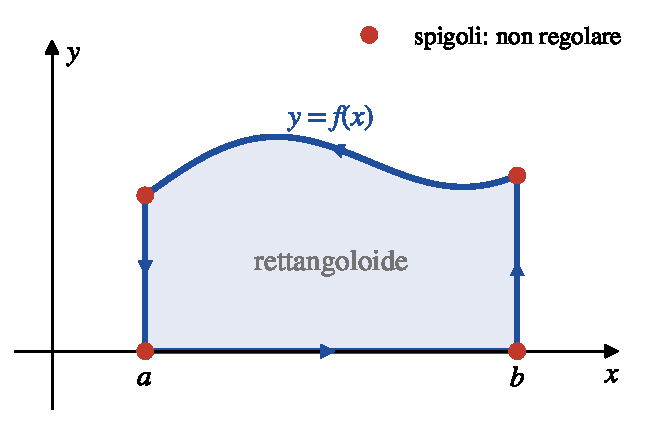
\includegraphics[width=0.6\linewidth]{figure/fig_10}\caption{Il bordo di un rettangoloide, percorso in verso antiorario, è una curva chiusa regolare a tratti: è formato da tre segmenti e dal grafico di $f$, e negli spigoli non è regolare (andamento qualitativo).}\label{fig:10}\end{figure}

% [1:22:45]
\subsection{Esempio 7: elica}

L'elica in $\mathbb{R}^3$ è la curva
\[
\varphi\colon\begin{cases} x(t)=R\cos t\\ y(t)=R\sin t\\ z(t)=t\end{cases}
\qquad t\in[0,2\pi]\qquad(R>0).
\]
% [1:24:38]
Per trovarne le equazioni si pensa a una molla: guardandola dall'alto si vede una
circonferenza, quindi le prime due componenti, nel piano $xy$, devono descrivere una
circonferenza; intanto la quota cresce ($z=t$), il punto sale e la curva non si chiude
(figura~\ref{fig:11}). È un esempio interessante perché usa ciò che si sa nel piano per
costruire una parametrizzazione in $\mathbb{R}^3$;
% [1:26:03]
con $t\in[0,2\pi]$ l'elica fa un solo giro.

\begin{itemize}
\item È regolare:
% [1:26:03]
$\varphi'(t)=(-R\sin t,\ R\cos t,\ 1)$ non è mai nullo, perché la derivata della terza
componente vale~$1$; anzi $|\varphi'(t)|=\sqrt{R^2+1}$.
\item Non è chiusa: $\varphi(0)=(R,0,0)\neq(R,0,2\pi)=\varphi(2\pi)$. Il dislivello
percorso dopo un giro completo, qui $2\pi$ (in generale $2\pi c$ se $z(t)=ct$), si chiama
\emph{passo} dell'elica.
\item È semplice (la terza componente $t$ è iniettiva, come osservato per la cuspide).
\end{itemize}
Il versore tangente è
\[
T(t)=\frac{\varphi'(t)}{|\varphi'(t)|}=\frac{1}{\sqrt{R^2+1}}\,(-R\sin t,\ R\cos t,\ 1).
\]

\begin{figure}[htbp]\centering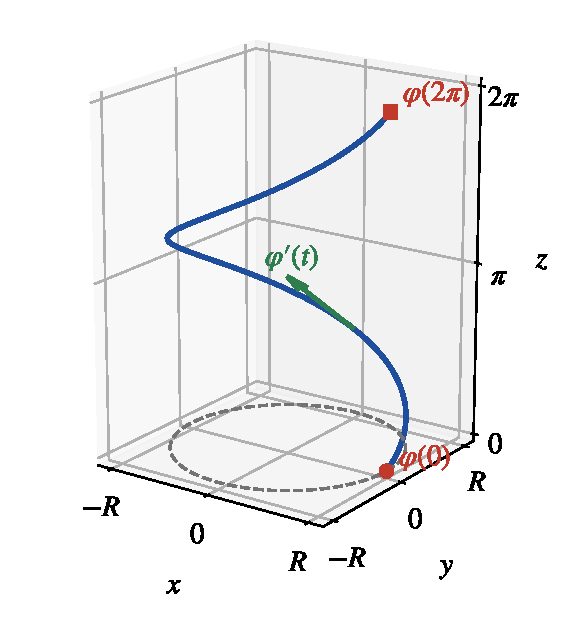
\includegraphics[width=0.6\linewidth]{figure/fig_11}\caption{Elica $\varphi(t)=(R\cos t,\ R\sin t,\ t)$, $t\in[0,2\pi]$, con $R=1$: vista dall'alto, cioè proiettata sul piano $xy$ (tratteggio), è una circonferenza; in verde un vettore tangente $\varphi'(t)$.}\label{fig:11}\end{figure}

% [1:26:03]
\paragraph{Osservazione.} Negli esercizi le equazioni parametriche non saranno date:
quando si dovrà integrare lungo una curva, o lungo il bordo di un insieme (che sarà una
curva), bisognerà saperla parametrizzare da soli, come si è fatto qui per l'elica.

% DUBBI:
% - p. 1: «La curva è il SOSTEGNO => Insieme dei p.ti» contraddice la definizione (la curva è
%   la legge oraria, il sostegno ne è il codominio): reso come «ciò che chiamiamo curva, il
%   disegno, è il sostegno», secondo l'audio [0:09:59].
% - p. 1: «Ci sono infinite traiettorie che hanno come codominio questa curva»: termini
%   scambiati; reso come «infinite curve (leggi orarie) hanno come codominio questa
%   circonferenza», come nell'audio [0:09:59].
% - p. 2, prima riga: «2 circonferenze [?] 1, 2 ma i dom. sono diverse»: la parola illeggibile
%   potrebbe essere «phi» (phi_1, phi_2 dell'esempio di p. 2) oppure «percorse» (1 e 2
%   volte, audio [0:04:00]-[0:07:17]); il senso (stesso disegno, domini diversi) è lo stesso.
% - p. 2: la definizione di curva negli appunti usa R^m e (x_1,...,x_m); uniformato a R^n come
%   nel resto degli appunti e nell'audio [0:14:20].
% - p. 3: gli esempi gamma_1, gamma_2, gamma_3 sono le curve phi_1, phi_2 di p. 2 e la phi_3
%   dell'audio [0:30:06]: notazione uniformata a phi.
% - p. 3: «La circonferenza è quindi una curva non semplice» è falso per phi_1 (su [0,2pi] è
%   semplice): riferito a phi_2 su [0,3pi], come nell'audio [0:28:41].
% - p. 6: la curva dell'Esempio 4 è scritta «f(t)» (probabile phi manoscritta letta dall'OCR
%   come f; l'audio [1:01:23] dice phi): rinominata phi, anche per non confonderla con la f
%   dell'Esempio 1.
% - p. 6: «Esempio (come la alpha [?]) di curva non semplice ma regolare»: interpretato come
%   richiamo alla circonferenza phi_2 per l'audio [1:09:18] («succedeva pure con la
%   circonferenza»); potrebbe anche alludere alla forma della curva, simile a una alpha.
% - p. 6: esplicitati il confronto phi(-a) != phi(a) sulla seconda componente e il valore 1/3
%   della prima componente di phi' in t=-2/3 (negli appunti solo «sono diversi» / «No»).
% - p. 7: «Non è regolare => Punto di non deriv.»: gamma è derivabile anche in t=0, ma
%   gamma'(0)=(0,0); la non derivabilità riguarda il sostegno (cuspide), come dice l'audio
%   [1:15:39]; aggiunta una precisazione tra parentesi.
% - p. 8: «È regolare, ~~orientata~~ [?] ma no»: parola cancellata e frammento illeggibile,
%   omessi; le proprietà dell'elica seguono l'audio [1:24:38]-[1:27:12]. R>0 non è scritto
%   negli appunti; phi'(t) e |phi'(t)| sono calcolati.
% - audio [0:20:27]-[0:21:13]: passaggio confuso su circuitazione e campi conservativi («se la
%   circuitazione è nulla è conservativo [...] prima sarà vero, poi andrà a falso»): reso in
%   forma generica con [?]. Probabile riferimento alla condizione rot F = 0, che basta solo su
%   domini opportuni (semplicemente connessi); per un campo continuo su un aperto, invece,
%   «circuitazione nulla su ogni curva chiusa» equivale sempre alla conservatività.
% - audio [0:33:26]-[0:34:50]: l'esempio (t,t^2) su [0,500] e [-50,50] è trascritto in modo
%   confuso; la motivazione («la prima componente t distingue gli istanti») è ricostruita.
% - audio [0:54:41]: «non sono mai uguali a meno che non si sia su 45 gradi» incomprensibile;
%   sostituito con l'argomento sugli estremi t=0, t=2pi.
% - audio [1:18:01]: «una ruota che scivola [...] senza attrito» corretto in «rotola senza
%   strisciare», il moto che genera la cicloide.
% - audio [0:42:09]: sulla trisezione il docente dice «è facile se l'angolo è multiplo di tre»,
%   che non è il criterio giusto (60° non si triseca con riga e compasso): omesso.
% - audio [1:27:12]: «pensate al rettangoloide [...] e questo mi darà la stessa ragione»:
%   chiusura del ragionamento incomprensibile, marcata [?].
% - audio [0:15:49]: l'esempio del moto discontinuo («piano H», «ABG») è trascritto in modo
%   confuso; parafrasato.
% - figure: fig_01-fig_09 e fig_11 ricostruiscono i disegni degli appunti (pp. 1-8), con
%   parametri scelti (a=1,25 in fig_07, r=1, R=1); fig_10 (rettangoloide) è uno schema
%   dall'audio [1:27:12], non presente negli appunti. Nessun ritaglio originale usato.
% - audio [0:44:45]-[0:47:47] (pausa, frasi allucinate) e ripetizioni in [0:58:03] ignorati.
